%!TEX root = ../sample.tex

\subsection{The POPP-Dirichlet}
\label{subsec:popd}

The C-POPP model requires the true positive rate $P^+$ and true negative rate $P^-$ to be specified in advanced in estimating the parameter $\lambda$ of a Poisson process. These are an extension of $\tau$ and $\xi$ where the rates provide a probability for a particular combination of binary detections coming from each sensor given the true event as shown in Eq. \ref{eq:joint_sensor_model_positive_event} and Eq. \ref{eq:joint_sensor_model_negative_event}.

To construct an observation model of $P^+$ and $P^-$, one needs to have both detections and the corresponding actual (non-)events as ground truth. Pre-processing involving expert interventions is typically required before the detections and their corresponding ground truth can be further used. Similarly to the POPP model, the C-POPP model requires the observation model to be accurate to avoid the posterior over $\lambda$ drifting away from the true posterior. If attaining an accurate observation model for the POPP model is a problem, then this becomes more challenging in the case of C-POPP model. This is because the training data needed to construct an observation model grows by a factor of two for each sensor involved.       

Analogously to the extension from the POPP model to the POPP-Beta model, we can expand the C-POPP observation model. In this case the observation models ($P^+$ and $P^-$) will follow Dirichlet distributions. The Dirichlet distribution is an appropriate distribution since $P^+$ and $P^-$ are the probabilities of categorical distributions which set the probabilities of multinomial distributions in Eq. \ref{eq:codependent_sensor_likelihood} and Dirichlet distributions provide a family of conjugate prior probability distributions for the multinomial distribution. The Dirichlet-multinomial conjugacy leads to an analytically tractable compound distribution which is called the Dirichlet-multinomial distribution, where the $\mathbf{p} = (p_1, \ldots, p_r)$ parameter in the multinomial distribution $Mult(\mathbf{d} \mid c, \mathbf{p})$ is randomly drawn from a Dirichlet distribution $Dir(\mathbf{p} \mid \boldsymbol{\zeta})$. 
\begin{equation}
	\label{eq:beta_binomial_revisit}
	\begin{tabular}{r@{ = }l}
        $P(\mathbf{d} \mid c, \boldsymbol{\zeta})$ & $\displaystyle\int P(\mathbf{d} \mid c, \mathbf{p}) ~ P(\mathbf{p} \mid \boldsymbol{\zeta}) ~d\mathbb S_r$ \\ [2ex]
        & $\displaystyle\int Mult(\mathbf{d} \mid c, \mathbf{p}) ~ Dir(\mathbf{p} \mid \boldsymbol{\zeta}) ~d\mathbb S_r$ \\ [2ex]
        & $DM((d_1, \ldots, d_r) \mid c, (\zeta_1, \ldots, \zeta_r))$
	\end{tabular}
\end{equation}
\noindent with $\mathbf{d} = (d_1, \ldots, d_r)$, $\boldsymbol{\zeta} = (\zeta_1, \ldots, \zeta_r)$, and $d\mathbb S_r$ denotes integrating $\mathbf{p}$ with respect to the $(r - 1)$ simplex\footnote{The support of the Dirichlet distribution is the $(r - 1)$-dimensional simplex $\mathbb S_r$; that is, all $r$ dimensional vectors which form a valid probability distribution}.

\begin{figure}[t!]
	\centering
	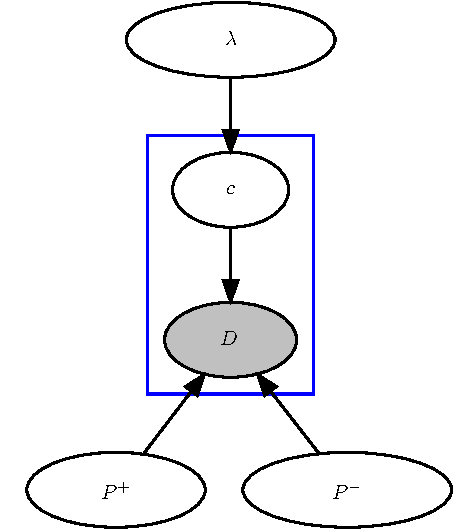
\includegraphics[width=0.35\textwidth]{./figures/popd-pics.pdf}
	\caption{Graphical representation of POPP-Dirichlet. Instead of having fixed estimated points for the (joint) sensor rates $P^+$ and $P^-$, they are represented by Dirichlet distributions in the POPP-Dirichlet.}
	\label{fig:gm_popp_dir}
	\vspace{-20pt}
\end{figure}

Given $m$ sensors, an observation model is now represented as two Dirichlet distributions: $Dir(P^+ \mid \boldsymbol{\zeta^+})$, and $Dir(P^- \mid \boldsymbol{\zeta^-})$ with $\boldsymbol{\zeta^+} = (\zeta^+_0, \ldots, \zeta^+_{(m^2)-1})$ and $\boldsymbol{\zeta^-} = (\zeta^-_0, \ldots, \zeta^-_{(m^2)-1})$. $\boldsymbol{\zeta^+}$ and $\boldsymbol{\zeta^-}$ set the overall shape of the Dirichlet priors, with each $\zeta_q$ term counting the number of times that particular combination of sensor detections were produced given a positive ($\boldsymbol{\zeta^+}$, $e=1$) or negative ($\boldsymbol{\zeta^-}$, $e=0$) detection.

Given a joint sensor model where its elements follow a Dirichlet density and several Dirichlet-multinomial distributions, which provide an unconditional distribution of $\mathbf{d}$, we replace Eq. \ref{eq:codependent_sensor_likelihood} with:  
\begin{equation}
	\label{eq:joint_dirichlet_multinomial_distribution}
    \begin{tabular}{r@{=}l}
		$P(\mathbf{D} \mid c)$ & $\sum\limits_{(\mathbf{e}^+, \mathbf{e}^-) \in \Sigma_c} DM(\mathbf{g}^+ \mid c, \boldsymbol{\zeta^+}) ~ DM(\mathbf{g}^- \mid (l - c), \boldsymbol{\zeta^-})$
	\end{tabular}
\end{equation}
\noindent with $\Sigma_c$ and $\mathbf{D}$ as defined in Section~\ref{subsec:cpop}.
% With a joint sensor model following the Dirichlet density, which is conjugated with multinomial distributions into a posterior predictive distribution shown in Eq. \ref{eq:joint_dirichlet_multinomial_distribution}, a graphical model is shown in Figure \ref{fig:gm_popp_dirichlet}.

The difference between the C-POPP model and the POPP-Dirichlet lies only in Eq. \ref{eq:codependent_sensor_likelihood} being replaced by \ref{eq:joint_dirichlet_multinomial_distribution} which is depicted by Figure \ref{fig:gm_popp_dir}. The difference makes the POPP-Dirichlet to be more conservative in estimating the posterior $P(\lambda \mid \mathbf{s})$ over $\lambda$ than the C-POPP model given a certain Dirichlet prior, and limited training data for the sensor model.

% \begin{figure}[t!]
% 	\centering
% 	\begin{tikzpicture}
% 	\tikzstyle{place}=[rectangle,draw=blue,thick,minimum size=5 mm]
% 	\tikzstyle{every label}=[black]
% 	\begin{scope}
%     \node[place](51)[xshift=30mm]{$(\zeta^+_0, \ldots, \zeta^+_{(m^2)-1})$};
%     \node[place](52)[right of=51, xshift=30mm]{$(\zeta^-_0, \ldots, \zeta^-_{(m^2)-1})$};
%     \node[place](41)[above of=51, yshift=3mm]{$(E^+_0, \ldots, E^+_{(m^2)-1})$} edge[pre](51);
%     \node[place](42)[above of=52, yshift=3mm]{$(E^-_0, \ldots, E^-_{(m^2)-1})$} edge[pre](52);
%     \node[place](31)[above of=41, xshift=-30mm, yshift=3mm]{$S_{1i}$} edge[pre](41) edge[pre](42);
% 	\node[place](32)[right of=31, xshift=20mm]{$S_{2i}$} edge[pre](41) edge[pre](42);
% 	\node[place](33)[right of=32, xshift=10mm]{$\ldots$} edge[pre](41) edge[pre](42);
% 	\node[place](34)[right of=33, xshift=15mm]{$S_{(m-1)i}$} edge[pre](41) edge[pre](42);
% 	\node[place](35)[right of=34, xshift=22mm]{$S_{mi}$} edge[pre](41) edge[pre](42);
% 	\node[place](21)[above of=33]{$X_i$} edge[post](31) edge[post](32) edge[post](33) edge[post](34) edge[post](35);
% 	\node[place](11)[above of=21]{$\lambda$} edge[post](21);
% 	% \node[place](01)[above of=11]{$\alpha, \beta$} edge[post](11);
% 	\end{scope}
% 	\end{tikzpicture}
% 	\caption{Graphical representation of the POPP-Dirichlet.}
% 	\label{fig:gm_popp_dirichlet}
% \end{figure}